\vspace{-4em}
\section*{Abstract}
\sloppy

  Se presenta una aplicación en Google Earth Engine para monitorear la relación entre anomalías de temperatura superficial del mar (TSM) en la zona ENSO 1+2 y la dinámica de la cobertura agrícola en la costa peruana. La cobertura se delimita con un clasificador Random Forest entrenado sobre embeddings de AlphaEarth Foundations y etiquetas de cultivos derivadas de Sentinel-2/L2A, reduciendo la dependencia de campo. Con la máscara obtenida se construyen series NDVI y se analizan frente a anomalías TSM NOAA en una ventana de seis meses, cubriendo 15 años. GitHub Actions automatiza la ingesta de ICEN-IGP, habilitando interoperabilidad y análisis distrital.

  \subsection*{\textbf{Keywords:}}
  \textit{GEE, RandomForest, AlphaEarth V1, NOAA, Sentinel-L2A, NDVI, 1+2 ENSO, GitHub}

  \subsection*{\textbf{Code Metadata:}}
  \begin{table}[H]
    \scriptsize
    \setlength{\tabcolsep}{4pt}
    \begin{tabular}{p{0.48\textwidth}p{0.48\textwidth}}
      \hline
      \textbf{Current code version} & v1.0.0 \\

%       \textbf{Permanent link to code/repository
% used for this code version} & \url{https://github.com/your-repo/your-project} \\

      \textbf{Permanent link to Reproducible Capsule} & \url{https://interopclassifierrf.projects.earthengine.app/view/utp-alphaclass-tsm-ndvi} \\

      \textbf{Legal Code License} & - \\

      \textbf{Code versioning system used} & Git on GEE \\

      \textbf{Software code languages, tools, and services used} & JavaScript (GEE), Python (GitHub Actions) \\

      \textbf{Compilation requirements, operating environments, and dependencies} & Google Earth Engine account, GitHub account, Python environment for GitHub Actions \\

      \textbf{Link to developer documentation/manual} & \url{https://github.com/1nfinit0/informeTecnicoNDVIvsTSM/blob/master/informeTecnicoEEUTP.pdf} \\

      \textbf{Support email for questions} & \url{hsluis4326@gmail.com} \\
      \hline
    \end{tabular}
    \caption{Code metadata}
  \end{table}

\begin{multicols}{2}
  \section{Introducción}

    La agricultura de precisión es una práctica que busca optimizar el uso de recursos y mejorar la productividad agrícola mediante el uso de tecnologías avanzadas. En los últimos años estas tecnologías son cada vez más accesibles y los recursos computacionales necesarios para calcular los productos de estas tecnologías son más libres de uso. Dentro de estos productos se encuentra la clasificación de cobertura agrícola, el registro de la dinámica de temperatura de la superficie del mar (TSM), los índices de vegetación, entre otros. Este estudio presenta una aplicación realizada sobre Google Earth Engine (GEE) que permite la integración de estos productos con el objetivo de monitorear históricamente la relación entre las anomalías de la TSM en la zona 1+2 ENSO y la respuesta de la cobertura agrícola en la costa peruana. Para esto se utiliza un clasificador Random Forest entrenado sobre vectores de Satellite Embedding V1/ANUAL (AlphaEarth Foundations) con etiquetas de cultivos agrícolas obtenidos a través de impagenes de satelitales (Sentinel-L2A) en la zona de Lambayeque-Perú. Este flujo reduce sustancialmente la dependencia de datos de campo y tiempos de procesamiento respecto a métodos tradicionales basado en pixeles. A partir de tal máscara se construyen series temporales del índice diferencial normalizado de vegetación (NDVI) y se relacionan con las anomalías de la TSM (NOAA) en la zona 1+2 ENSO medias de una ventana temporal de 6 meses previas al mes de análisis ofreciendo una perspectiva de tal comportamiento en los últimos 15 años. Una contribución central de este trabajo es un puente de interoperabilidad de datos que se implementa mediante Github Actions que ingesta de manera periódica y automatizada datos de fuentes externas (ICEN-IGP) Instituto Geofísico del Perú. La plataforma resultante permite el análisis a nivel distrital, bajo demanda y a través de una interfaz cartográfica interactiva ofreciendo de esta manera un marco replicable para el monitoreo climático-agrícola en entornos costeros con limitaciones en datos de campo y recursos computacionales.

    \begin{figure}[H]
      \centering
      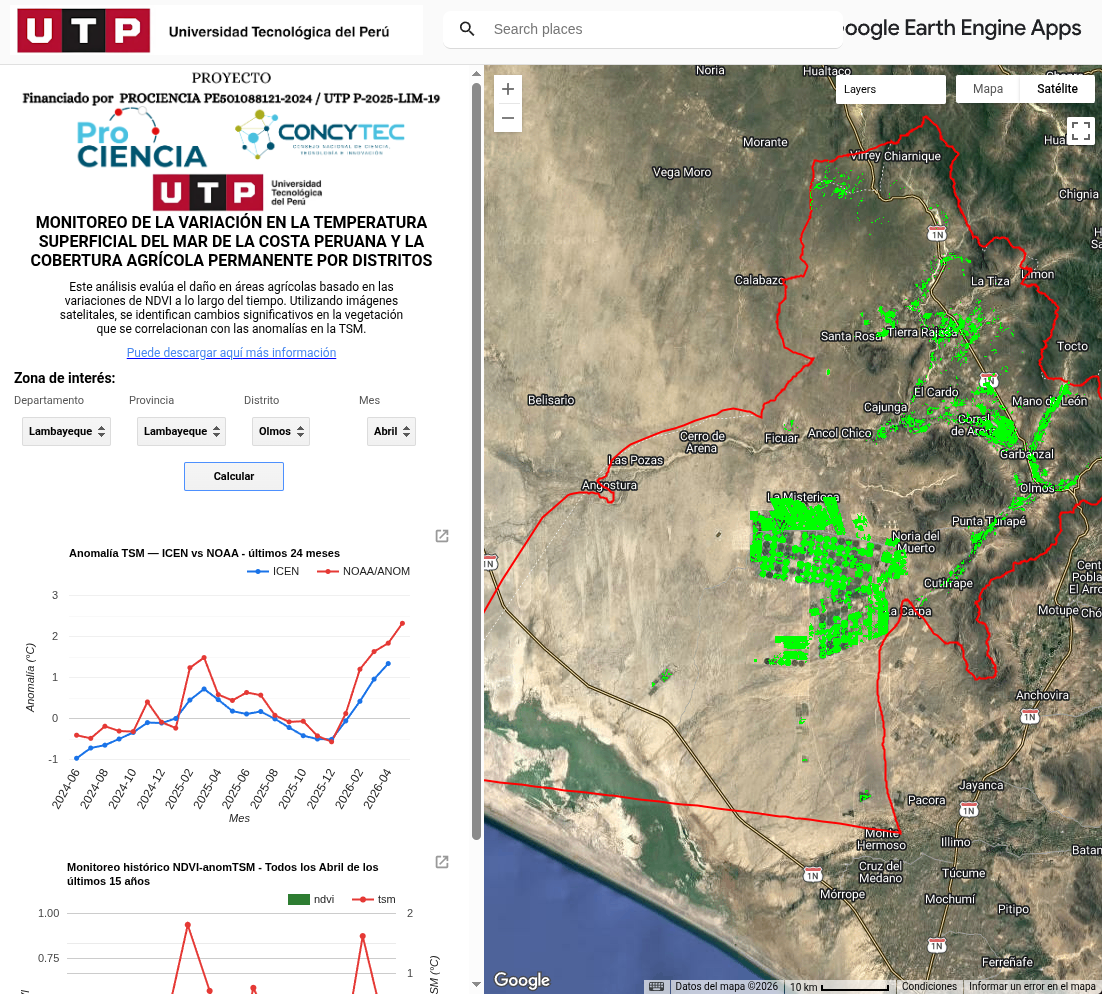
\includegraphics[width=0.45\textwidth]{assets/gee/gee.png}
      \caption{Interfaz de la aplicación desarrollada en Google Earth Engine, se muestra la capa de cobertura agrícola (verde) y a la izquierda el panel con las opciones de análisis y gráficos de monitoreo.}
    \end{figure}

    \section{Materiales y Métodos}

      El desarrollo de la aplicación, por sus características de integración de datos y análisis geoespacial, se estructura en partes independientes y modulares. Estas se integran para ofrecer una funcionalidad eficiente y robusta para el usuario. Además, facilitan el mantenimiento y la escalabilidad del código. A continuación, se describen los materiales necesarios para su desarrollo:

      \begin{itemize}[leftmargin=*]
        \item \textbf{Google Earth Engine (GEE):} Plataforma de análisis geoespacial en la nube que permite el procesamiento de grandes cantidades de datos satelitales y geoespaciales. Se utiliza para desarrollar y alojar la aplicación, realizar el análisis de datos y generar visualizaciones interactivas.
        \item \textbf{GitHub Actions:} Herramienta de integración y entrega continua (CI/CD) que permite automatizar flujos de trabajo. Se utiliza para implementar un puente de interoperabilidad que ingesta datos periódicamente desde fuentes externas (ICEN-IGP).
        \item \textbf{Python:} Lenguaje de programación utilizado para escribir los scripts de automatización en GitHub Actions.
        \item \textbf{JavaScript-GEE:} Lenguaje de programación utilizado para desarrollar la aplicación en Google Earth Engine, en este caso GEE ofrece un el lenguaje con ajustes específicos para el desarrollo dentro de la plataforma.
        \item \textbf{Datos de anomalía TSM NOAA:} Anomalías de la temperatura superficial del mar (TSM) en la zona 1+2 ENSO obtenidos del dataset Optimum Interpolation Sea Surface Temperature en GEE (NOAA CDR OISST v02r01).
        \item \textbf{Datos de anomalía TSM ICEN:} Anomalías de la temperatura superficial del mar (TSM) en áreas costeras peruanas obtenidos del Índice Costero de El Niño (ICEN) del Instituto Geofísico del Perú (IGP) que se ingesta de manera automatizada mediante GitHub Actions como asset.
        \item \textbf{Random Forest:} Modelo de machine learning utilizado para la clasificación de la cobertura agrícola a partir de los vectores de Satellite Embedding V1/ANUAL (AlphaEarth Foundations).
        \item \textbf{Satellite Embedding V1/ANUAL (AlphaEarth Foundations):} Conjunto de vectores de embedding en Google Earth Engine con identificador de datos: \texttt{GOOGLE/SATELLITE\_EMBEDDING/V1/ANNUAL}, versión 1.1, provisto por Google Earth Engine y Google DeepMind. Representa características espectrales y temporales de imágenes satelitales caracterizadas en 64 bandas con resolución temporal continua y está disponible para el periodo \texttt{2017-01-01T00:00:00Z}--\texttt{2025-01-01T00:00:00Z}. Se utiliza como insumo para entrenar el clasificador Random Forest.
        \item \textbf{Etiquetas de entrenamiento:} Etiquetas digitalizadas manualmente en el software QGIS a partir de imágenes satelitales Sentinel-2/L2A con periodo de adquisición \textit{2024-01-01 a 2024-02-01} que identifican áreas de cultivos agrícolas en la zona de Lambayeque-Perú, utilizadas para entrenar el modelo de clasificación.
        \item \textbf{Índice NDVI:} Índice diferencial normalizado de vegetación calculado a partir de las imágenes satelitales para monitorear la dinámica de la cobertura agrícola.
      \end{itemize}

    \subsection{Clasificación de la cobertura agrícola}

      Para la clasificación de la cobertura agrícola se utiliza un modelo de Random Forest con 200 árboles de decisión entrenado sobre los vectores de Satellite Embedding V1/ANUAL (AlphaEarth Foundations) con etiquetas de cultivos agrícolas obtenidos a través de imágenes de satelitales (Sentinel-2/L2A) en la zona de Lambayeque-Perú. Se generaron más de 300 polígonos de muestra representativos y balanceados en dos clases: cobertura agrícola y no agrícola.

      \begin{figure}[H]
        \centering
        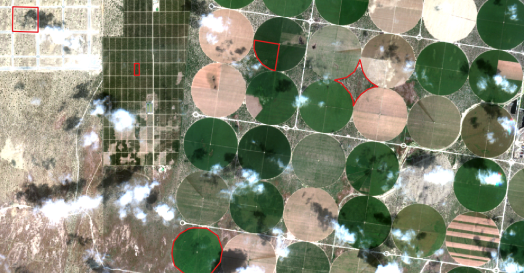
\includegraphics[width=0.45\textwidth]{assets/gee/etiquetas.png}
        \caption{Máscara de cobertura agrícola realizada de manera manual mediante software QGIS a partir de imágenes satelitales Sentinel-2/L2A, se muestra la zona de Lambayeque-Perú con áreas etiquetadas como cultivos agrícolas y no agrícolas.}
      \end{figure}

      El modelo es entrenado con el 70\% de los polígonos de referencia y evaluado con el 30\% restante. La división se realizó a nivel de polígono y antes de la extracción de muestras espectrales con el fin de evitar fuga de datos por autocorrelación espacial, píxeles pertenecientes a un mismo polígono comparten características casi idénticas entre sí, por lo que una división a nivel de píxel permitiría que el modelo fuese evaluado con información redundante ya vista durante el entrenamiento, inflando artificialmente las métricas de desempeño. Con la división corregida por polígono se obtuvo la matriz de confusión mostrada en el Cuadro 2.

      \begin{table}[H]
        \centering
        \scriptsize
        \setlength{\tabcolsep}{4pt}
        \renewcommand{\arraystretch}{1.3}
        \begin{tabular}{lcc}
          \hline
          & \textbf{Agrícola} & \textbf{No Agrícola} \\[2pt]
          \hline
          \textbf{Real: Agrícola}    & 3216 & 518    \\
          \textbf{Real: No Agrícola} & 119   & 7352 \\
          \hline
        \end{tabular}
        \caption{Matriz de confusión del modelo RF. División entrenamiento/validación realizada a nivel de polígono; evaluación calculada sobre n=11 205 píxeles de validación, provenientes de los polígonos no usados en entrenamiento. Se observa que el modelo clasifica correctamente 3216 píxeles de cobertura agrícola y 7352 píxeles de no agrícola, mientras que comete 518 falsos negativos y 119 falsos positivos.}
        \label{tab:matriz-confusion}
      \end{table}

      La precisión global obtenida fue de 94.32\%, con un coeficiente Kappa de 0.869, lo que indica un desempeño sustancial y confiable del modelo en la clasificación de cobertura agrícola (Cuadro 3).

      \begin{table}[H]
        \centering
        \scriptsize
        \setlength{\tabcolsep}{4pt}
        \renewcommand{\arraystretch}{1.3}
        \begin{tabular}{lccc}
          \hline
          \textbf{Clase} & \textbf{Usuario} & \textbf{Producto} & \textbf{F1-Score} \\
          \hline
          \textbf{Agrícola}     & 96.34\% & 86.13\% & 0.910 \\
          \textbf{No agrícola}  & 93.42\% & 98.41\% & 0.958 \\
          \hline
        \end{tabular}
        \caption{Métricas de desempeño del modelo RF por clase, calculadas a partir de la matriz de confusión. La precisión de usuario indica la confiabilidad de las predicciones positivas, mientras que la precisión de producto indica la proporción de píxeles reales correctamente clasificados. El F1-Score es la media armónica entre ambas métricas.}
        \label{tab:metricas-desempeño}
      \end{table}

      Se observa una menor sensibilidad para la clase Cultivo (86.13\%), lo que sugiere que el modelo tiende a subestimar de forma conservadora la extensión real de cobertura agrícola, mientras que su precisión para dicha clase es alta (96.43\%), es decir, las predicciones positivas de cultivo son mayormente confiables.

      Adicionalmente, se calcularon los errores de omisión y comisión por clase, métricas estándar en la evaluación de clasificaciones de cobertura de suelo en teledetección, las cuales complementan la información de la matriz de confusión (Cuadro 2).

      \begin{table}[H]
        \centering
        \scriptsize
        \setlength{\tabcolsep}{4pt}
        \renewcommand{\arraystretch}{1.3}
        \begin{tabular}{lcc}
          \hline
          \textbf{Clase} & \textbf{Error Omisión} & \textbf{Error Comisión} \\
          \hline
          \textbf{Agrícola}     & 13.87\% & 3.57\%  \\
          \textbf{No agrícola}  & 6.58\%  & 1.59\%  \\
          \hline
        \end{tabular}
        \caption{Errores de omisión y comisión por clase del modelo RF, explican la proporción de falsos negativos y falsos positivos respectivamente, complementando la información de la matriz de confusión.}
        \label{tab:errores-omision-comision}
      \end{table}

      El error de omisión más alto corresponde a la clase Cultivo (13.87\%), lo que indica que una proporción de los píxeles agrícolas reales no fue detectada por el modelo (falsos negativos), consistente lo observado para esta clase (86.13\%, Cuadro 3). En contraste, el error de comisión es bajo para ambas clases <4\%, indicando que las predicciones positivas del modelo son mayormente confiables.

      \subsection{Aplicación del modelo a otras zonas geográficas}

      Es posible aplicar el modelo a un distrito fuera de su área de entrenamiento, aunque considerando zonas geográficamente similares. Es razonable esperar que los embeddings capturen señales comparables entre ambas zonas sin que sea necesario entrenar un modelo distinto por cada distrito. Sin embargo, al no contar con datos de validación de los resultados la salida debe interpretarse como una demostración de la capacidad del modelo de aplicarse a otras zonas y no como una exactitud cuantificada. Es posible extender la validación a otros distritos mediante la incorporación de etiquetas de entrenamiento de estas áreas, nuevas y geográficamente distintas etiquetas de entrenamiento enriquecerían el modelo.

      \begin{figure}[H]
        \centering
        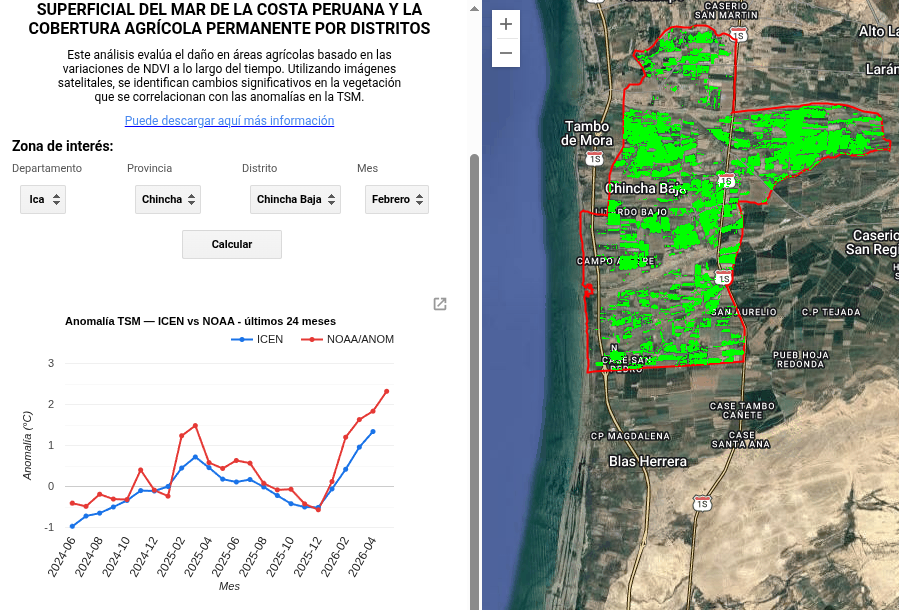
\includegraphics[width=0.45\textwidth]{assets/gee/mascara.png}
        \caption{Máscara de cobertura agrícola del distrito de Chincha Baja (Ica), obtenida al aplicar, sin reentrenamiento, el modelo entrenado con etiquetas agrícolas de Lambayeque, Perú, obtenidas a través de imágenes satelitales (Sentinel-2/L2A), sobre vectores de Satellite Embedding V1/ANUAL (AlphaEarth Foundations). Resultado ilustrativo de la capacidad de generalización del modelo a otros valles costeros.}
      \end{figure}

      \subsection{Registro del monitoreo de la relación entre anomalías de TSM y dinámica agrícola}

        A partir de la máscara de cobertura agrícola obtenida, se construyen series temporales del Índice de Vegetación de Diferencia Normalizada (NDVI) y de las anomalías de la Temperatura Superficial del Mar (TSM) en la región ENSO 1+2, utilizando el promedio de una ventana temporal de seis meses previa al mes de análisis. La visualización presenta el comportamiento histórico de ambas variables para el período 2009–2024, con el propósito de facilitar su comparación temporal.

        \begin{figure}[H]
          \centering
          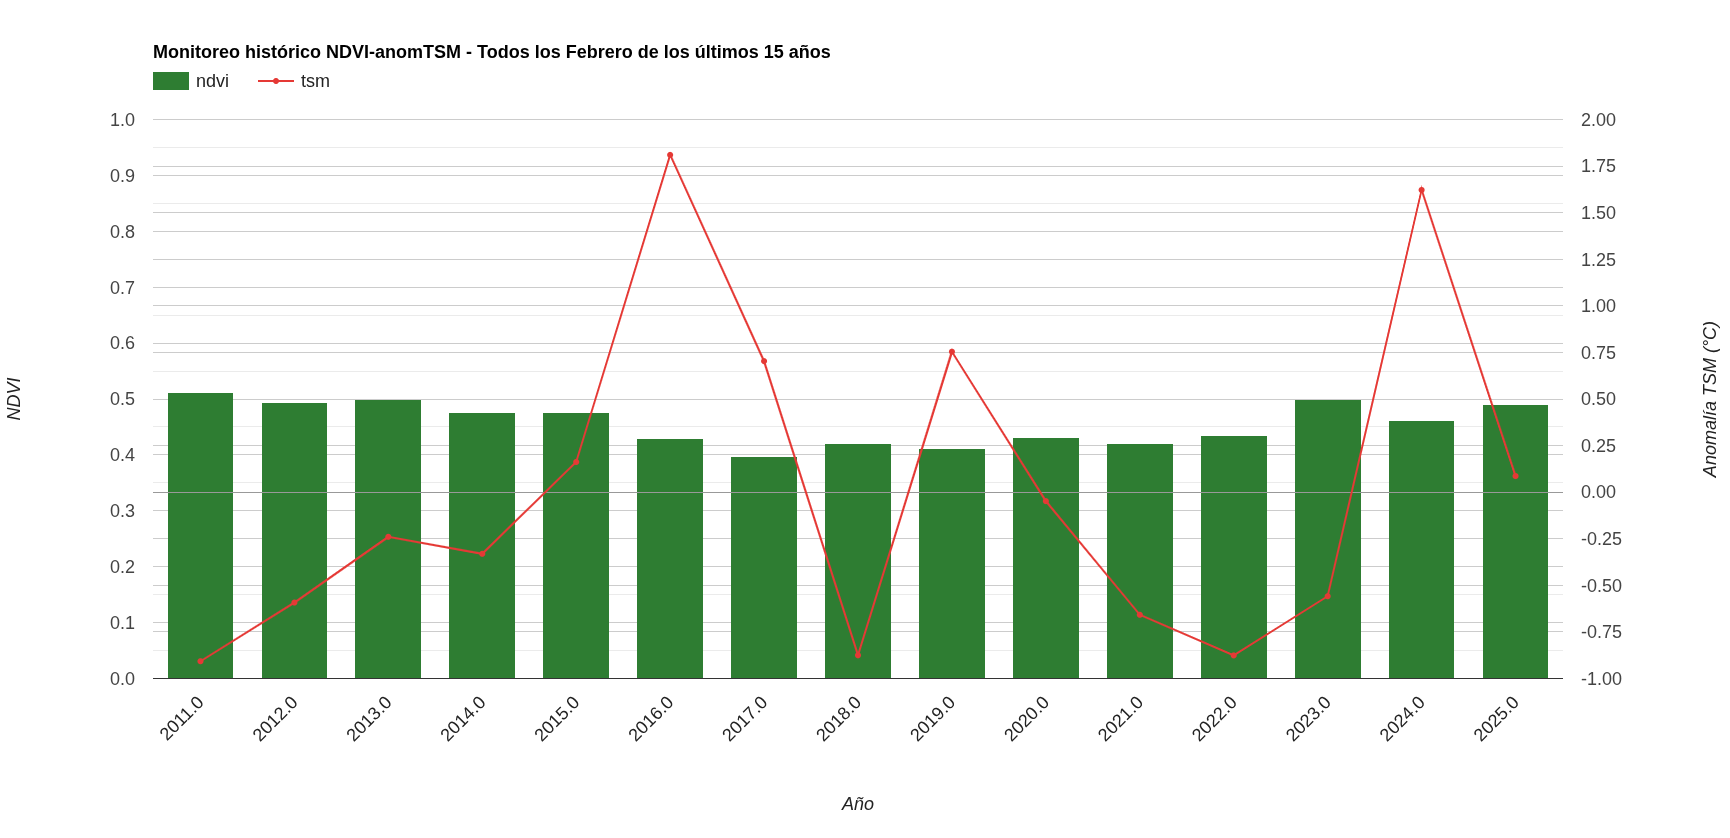
\includegraphics[width=0.45\textwidth]{assets/gee/anomTSM-NDVI.png}
          \caption{Visualización comparativa para el mes de febrero en el distrito de Chincha Baja (Ica). Se muestran los valores de NDVI y las anomalías de la TSM correspondientes a los meses de febrero del período 2009–2024. La figura tiene fines de comparación visual y no representa una medida de correlación estadística.}
        \end{figure}

        \subsection{Automatización de la ingesta periódica de datos externos}

          Intentar mantener actualizada la aplicación con datos externos provenientes de fuentes como el Instituto Geofísico del Perú (IGP) puede convertirse en una tarea repetitiva si se realiza manualmente. Para automatizar este proceso, se implementó un puente de interoperabilidad mediante GitHub Actions, este ejecuta un flujo de trabajo diario que descarga la información del Índice Costero El Niño (ICEN), la procesa y actualiza los datos utilizados por la aplicación.

          La autenticación con Google Earth Engine se realiza mediante una cuenta de servicio, cuyas credenciales se almacenan de forma segura como GitHub Secrets, esto permite que el flujo de trabajo publique automáticamente los activos generados sin exponer información sensible.

          Como limitación, el flujo de trabajo depende de la estabilidad de la estructura y disponibilidad de los recursos publicados por el IGP. Cambios en el enlace de acceso, el formato del archivo o su estructura pueden provocar fallos en la actualización automática, por lo que se recomienda implementar mecanismos de validación y notificación para detectar oportunamente este tipo de incidencias.

          Este flujo permite contar con datos oficiales y actualizados de las anomalías de la TSM en áreas costeras peruanas, lo que enriquece el análisis y monitoreo ofrecido por la aplicación. Con el desarrollo de la herramienta es posible resolver la problemática de monitoreo climático-agrícola en entornos costeros con limitaciones en datos de campo y recursos computacionales, de ser necesario se pueden integrar otros productos como índices de humedad, índices de estrés hídrico, entre otros, logrando así resultados como el siguiente:

          \begin{figure}[H]
            \centering
            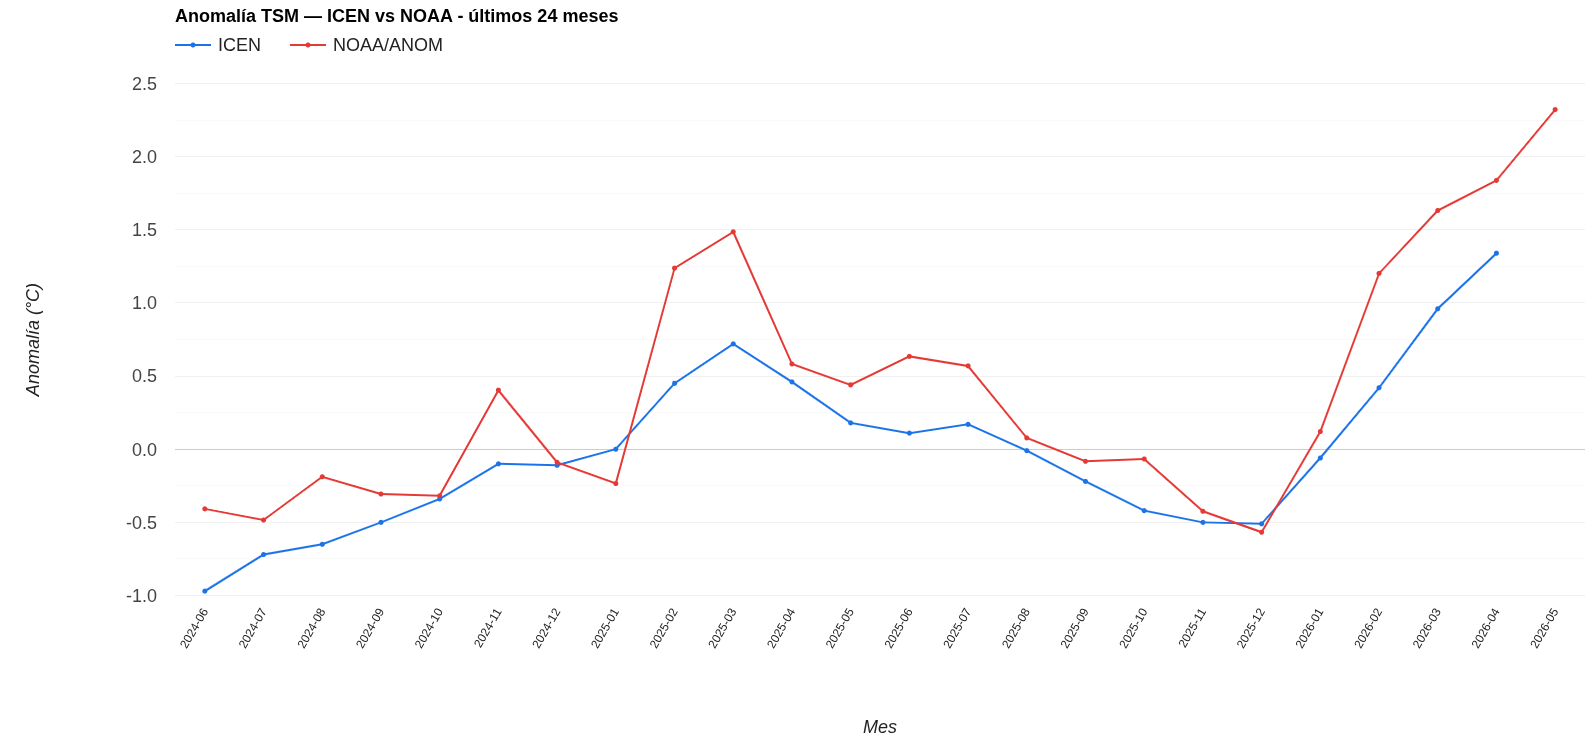
\includegraphics[width=0.45\textwidth]{assets/gee/anom.png}
            \caption{Comparación visual entre las series temporales de anomalías de TSM provenientes de NOAA e ICEN. Aunque ambas presentan diferencias en magnitud debido a sus metodologías de generación, se aprecia una tendencia temporal similar. Esta comparación tiene carácter ilustrativo y constituye una verificación visual del funcionamiento del flujo de ingesta, sin representar una validación estadística de la equivalencia entre ambas series. muestra el registro de las medias de anomalías de TSM (NOAA) de color rojo y las anomalías de TSM (ICEN) de color azul. Las ubicaciones espaciales de toma de datos em ambos datasets puede ser diferente pero su tendencia guarda similitud.}
          \end{figure}

          La fuente de oficial de información, Índice Costero El Niño (ICEN), puede presentar un retraso de varios meses respecto a la fecha de actual. Para mantener la capacidad de monitoreo de las condiciones oceánicas más recientes, la aplicación incorpora de manera complementaria el conjunto de datos OISST (NOAA), el cual se actualiza diariamente según especificaciones. De esta forma, el ICEN constituye la referencia oficial para el análisis histórico, mientras que OISST permite disponer de información correspondiente al período más reciente hasta que el IGP publique la actualización oficial del índice.

          Finalmente, los datos del ICEN son almacenados en Google Earth Engine como una FeatureCollection de tipo tabular, donde cada registro representa una observación mensual del índice. La estructura del asset incluye los campos yy (año), mm (mes) e icen (valor del Índice Costero El Niño). Esto permite realizar consultas temporales directamente desde Earth Engine e integrarlo con los análisis de series temporales desarrollados por la aplicación.

        \section{Funcionalidades}

          Para un usuario final, la aplicación ofrece una interfaz interactiva que permite seleccionar el área de interés para conocer la tendencia actual de la anomalía de la temperatura superficial del mar y como históricamente tal área a respondido a estas anomalías a través del índice NDVI.

          \subsection{Descripción}

            Muestra la información relevante acerca del fin del proyecto y un enlace a su manual.

            \begin{figure}[H]
              \centering
              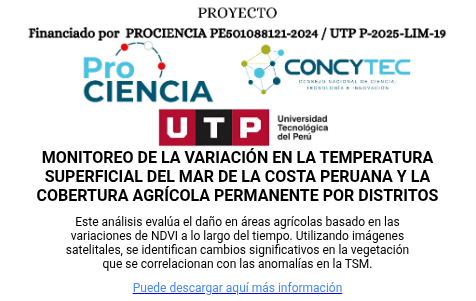
\includegraphics[width=0.45\textwidth]{assets/gee/descripcion.png}
              \caption{Título del proyecto, entidades responsables, descripción del proyecto y enlace al manual.}
            \end{figure}

          \subsection{Selección de área de interés}

            Se construyó un panel de selección de área de interés que lista mediante un formulario desplegable entidades geográficas asociadas al orden político-administrativo a nivel de distritos y un mes de análisis permitiendo capturar los parámetros necesarios para el cálculo del producto de monitoreo.

            \begin{figure}[H]
              \centering
              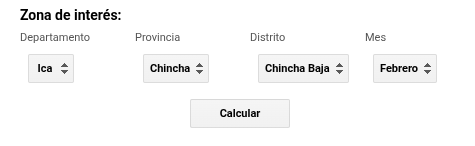
\includegraphics[width=0.45\textwidth]{assets/gee/form.png}
              \caption{Formulario de selección de área de interés y mes de análisis.}
            \end{figure}

          \section{Impacto}

            La aplicación desarrollada ofrece un marco replicable para el monitoreo climático-agrícola en entornos costeros con limitaciones en datos de campo y recursos computacionales. Al integrar datos de anomalías de TSM de distintas fuentes con la dinámica de la cobertura agrícola en demanda del usuario, se proporciona una herramienta valiosa para agricultores, investigadores y tomadores de decisiones que buscan comprender mejor la relación entre el clima y la agricultura en la costa peruana. Además, la automatización de la ingesta de datos externos garantiza que la aplicación se mantenga actualizada mejorando su utilidad a futuro.

          \section{Limitaciones y futuras mejoras}

            La generación de etiquetas de entrenamiento a partir de imágenes satelitales puede introducir un "sesgo geográfico "que puede limitar la clasificación a áreas con características similares como altitud, tipo de cultivo, entre otros. Para evitar esto es posible diversificar las etiquetas de muestra generadas de manera que cubran una mayor variedad de estas características.

            Por otro lado, al relacionarla con las anomalías de la temperatura superficial del mar (TSM) en la zona 1+2 ENSO el aprovechamiento de esta información se limita a las zonas costeras donde mayor es la influencia de estas anomalías, para mejorar esto es posible integrar otros productos como índices de humedad, índices de estrés hídrico, etc, que permitan ofrecer un análisis más completo de la relación entre el clima y la agricultura en distintas zonas del país.

  \end{multicols}
